% Plantilla común para figuras redibujadas (fig-NN-desc.tex).
% Copiar entera y sustituir solo el cuerpo entre las marcas "cuerpo de la figura".
% Compila tal cual en Overleaf o con scripts/tikz2svg.sh.
%
% NO añadir la opción "tikz" a standalone: parte cada tikzpicture (y cada
% \chemfig) en una página distinta y el SVG solo tendría la primera.
\documentclass[border=4pt]{standalone}
\usepackage[T1]{fontenc}
\usepackage{lmodern}            % base vectorial: sin fuente vectorial el texto sale en Type 3 y dvisvgm lo pierde
\usepackage[scaled=0.95]{helvet}% sans-serif tipo Helvetica, como la interfaz de Obsidian
\renewcommand{\familydefault}{\sfdefault}
\usepackage{amsmath,amssymb}
\usepackage{sansmath}\sansmath  % fórmulas en sans, a juego con el texto
\usepackage[version=4]{mhchem}  % \ce{A + B -> C}
\usepackage{chemfig}            % estructuras y esquemas de reacción
\usepackage{tikz}
\usetikzlibrary{arrows.meta,positioning,calc,shapes.geometric,decorations.pathmorphing,decorations.markings}
\usepackage{pgfplots}           % gráficas (cinética, curvas de valoración...)
\pgfplotsset{compat=1.18}

% ---- Estilo Apuntes.md --------------------------------------------------
% Paleta semántica (la misma que el CSS de Obsidian). Principios inspirados en
% figures4papers (ChenLiu-1996, CC BY-NC 4.0): se adoptan ideas, no código.
\definecolor{apAzul}{HTML}{0F4D92}       % anotaciones, estructura (el azul del autor)
\definecolor{apAzulClaro}{HTML}{3775BA}
\definecolor{apRojo}{HTML}{B64342}       % curvas y datos principales, importante (el rojo del autor)
\definecolor{apRojoClaro}{HTML}{E9A6A1}
\definecolor{apVerde}{HTML}{3B7D3B}      % definiciones, "positivo"
\definecolor{apVerdeClaro}{HTML}{AADCA9}
\definecolor{apGris}{HTML}{767676}       % apoyo: rejillas, referencias, líneas punteadas
\definecolor{apGrisClaro}{HTML}{CFCECE}
\definecolor{apNegro}{HTML}{272727}      % ejes y texto neutro

\tikzset{
  % sin "color=" global: pisaría los \color{...} de chemfig (estructuras en rojo, etc.)
  every picture/.append style={line width=0.9pt, >={Stealth[length=2.4mm]}},
  curva/.style={apRojo, line width=1.6pt},                  % la curva o el dato que importa
  curva secundaria/.style={apAzulClaro, line width=1.3pt},
  referencia/.style={apGris, dotted, line width=1pt},       % líneas guía (p. ej. y = 0)
  anotacion/.style={apAzul, font=\normalsize},              % texto escrito a mano alrededor del dibujo
  flecha/.style={->, apAzul, line width=1pt},
  implica/.style={-{Implies}, double, double distance=2pt, line width=0.8pt},
  marca/.style={circle, fill=apAzul, draw=white, line width=0.6pt, inner sep=1.8pt},
  resalte/.style={apAzul, line width=1pt},                  % círculos/óvalos que rodean algo
}
\pgfplotsset{
  apuntes/.style={
    axis lines=left, axis line style={line width=1pt, apNegro, -{Stealth[length=2.4mm]}},
    tick style={apNegro, line width=0.8pt}, tick align=outside,
    label style={font=\normalsize}, tick label style={font=\normalsize},
    every axis plot/.append style={curva},
    clip=false,
  },
}
\setchemfig{atom sep=2em, bond style={line width=0.9pt}}
% -------------------------------------------------------------------------

\begin{document}
% --- cuerpo de la figura ---
% Cromatografía en columna con sus partes (pág. 11)
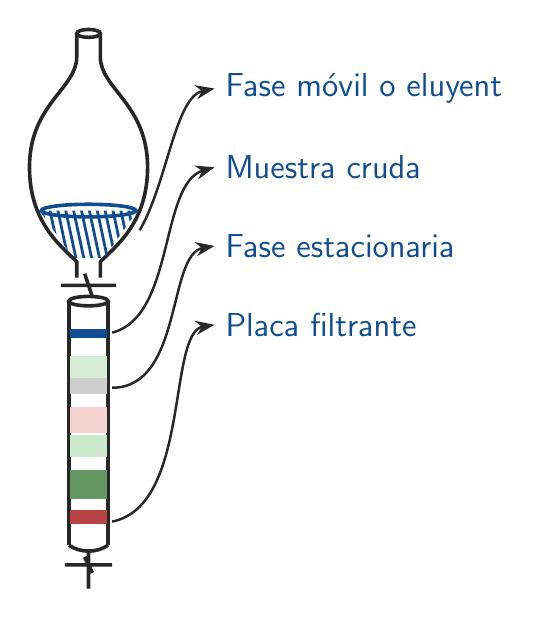
\begin{tikzpicture}[font=\large, line width=1.3pt]
  % depósito superior (ampolla)
  \draw[apNegro] (-0.15,4.3) -- (-0.15,4.0) .. controls (-0.15,3.6) and (-0.75,3.4) .. (-0.75,2.6)
        .. controls (-0.75,1.9) and (-0.35,1.6) .. (-0.15,1.4) -- (-0.15,1.2);
  \draw[apNegro] (0.15,4.3) -- (0.15,4.0) .. controls (0.15,3.6) and (0.75,3.4) .. (0.75,2.6)
        .. controls (0.75,1.9) and (0.35,1.6) .. (0.15,1.4) -- (0.15,1.2);
  \draw[apNegro] (0,4.3) ellipse (0.15 and 0.05);
  % fase estacionaria del depósito (rayado azul)
  \begin{scope}
    \clip (-0.62,2.05) -- (0.62,2.05) -- (0.2,1.45) -- (-0.2,1.45) -- cycle;
    \foreach \x in {-0.7,-0.6,...,0.7} \draw[apAzul, line width=1pt] (\x,2.1) -- (\x+0.15,1.4);
  \end{scope}
  \draw[apAzul] (0,2.05) ellipse (0.6 and 0.08);
  % llave intermedia
  \draw[apNegro] (-0.35,1.1) -- (0.35,1.1) (-0.05,1.25) -- (0.05,0.95);
  % columna
  \draw[apNegro] (-0.25,0.9) -- (-0.25,-2.2) (0.25,0.9) -- (0.25,-2.2);
  \draw[apNegro] (0,0.9) ellipse (0.25 and 0.06);
  \foreach \c/\y/\h in {apAzul/0.55/0.12, apVerdeClaro!50/0.2/0.3, apGrisClaro/-0.08/0.2, apRojoClaro!50/-0.45/0.32, apVerdeClaro!60/-0.8/0.28, apVerde!80/-1.25/0.36, apRojo/-1.75/0.18} {
    \fill[\c] (-0.23,\y) rectangle (0.23,{\y-\h});
  }
  \draw[apNegro] (-0.25,-2.2) .. controls (-0.1,-2.3) and (0.1,-2.3) .. (0.25,-2.2);
  % llave inferior
  \draw[apNegro] (0,-2.25) -- (0,-2.75) (-0.3,-2.45) -- (0.3,-2.45) (-0.05,-2.35) -- (0.05,-2.55);

  % etiquetas
  \node[anotacion, anchor=west, font=\large] (fm) at (1.6,3.6) {Fase móvil o eluyent};
  \node[anotacion, anchor=west, font=\large] (mc) at (1.6,2.6) {Muestra cruda};
  \node[anotacion, anchor=west, font=\large] (fe) at (1.6,1.6) {Fase estacionaria};
  \node[anotacion, anchor=west, font=\large] (pf) at (1.6,0.6) {Placa filtrante};
  \draw[->, apNegro, line width=0.9pt] (0.65,1.8) .. controls (1.0,2.4) and (1.1,3.5) .. (fm.west);
  \draw[->, apNegro, line width=0.9pt] (0.3,0.5) .. controls (1.1,0.7) and (0.9,2.4) .. (mc.west);
  \draw[->, apNegro, line width=0.9pt] (0.3,-0.2) .. controls (1.2,-0.2) and (1.0,1.5) .. (fe.west);
  \draw[->, apNegro, line width=0.9pt] (0.3,-1.9) .. controls (1.3,-1.7) and (1.0,0.5) .. (pf.west);
\end{tikzpicture}
% ---------------------------
\end{document}
